\documentclass{scrartcl}
\setcounter{tocdepth}{4}
\setcounter{secnumdepth}{4}
\usepackage[utf8]{inputenc}
\usepackage{graphicx} 
\usepackage{tabularx}
\usepackage{listings}
\usepackage{float}
\usepackage{pdfpages}
\usepackage{xcolor}
\usepackage{scrpage2}
\usepackage{tikz}
\usepackage[top=3.5cm, bottom=2.5cm, left=2.5cm, right=2.5cm,headheight=110pt]{geometry}

\title{Anperi}
\subtitle{Projektmanagement\\ Projektabschlussbericht \\  SS2018}
\author{Jannes Peters - 590252 \\ Adrian Kurth - 590289 \\ Jesse Nis Arff - 590245}
\date{22.06.2018}

\begin{document}

\maketitle
\newpage
\renewcommand\contentsname{Inhalt}
\tableofcontents{}
\newpage

\pagestyle{scrheadings}
\addtolength{\voffset}{-15pt}
\ihead{\textbf{Projektmanagement}}  
\chead{Projekt: Anperi \\ Dok.-Typ: Projektabschlussbericht}
\ohead{Datum: 22.06.2018}
\setheadsepline{0.4pt}

\section{Projektsteckbrief}
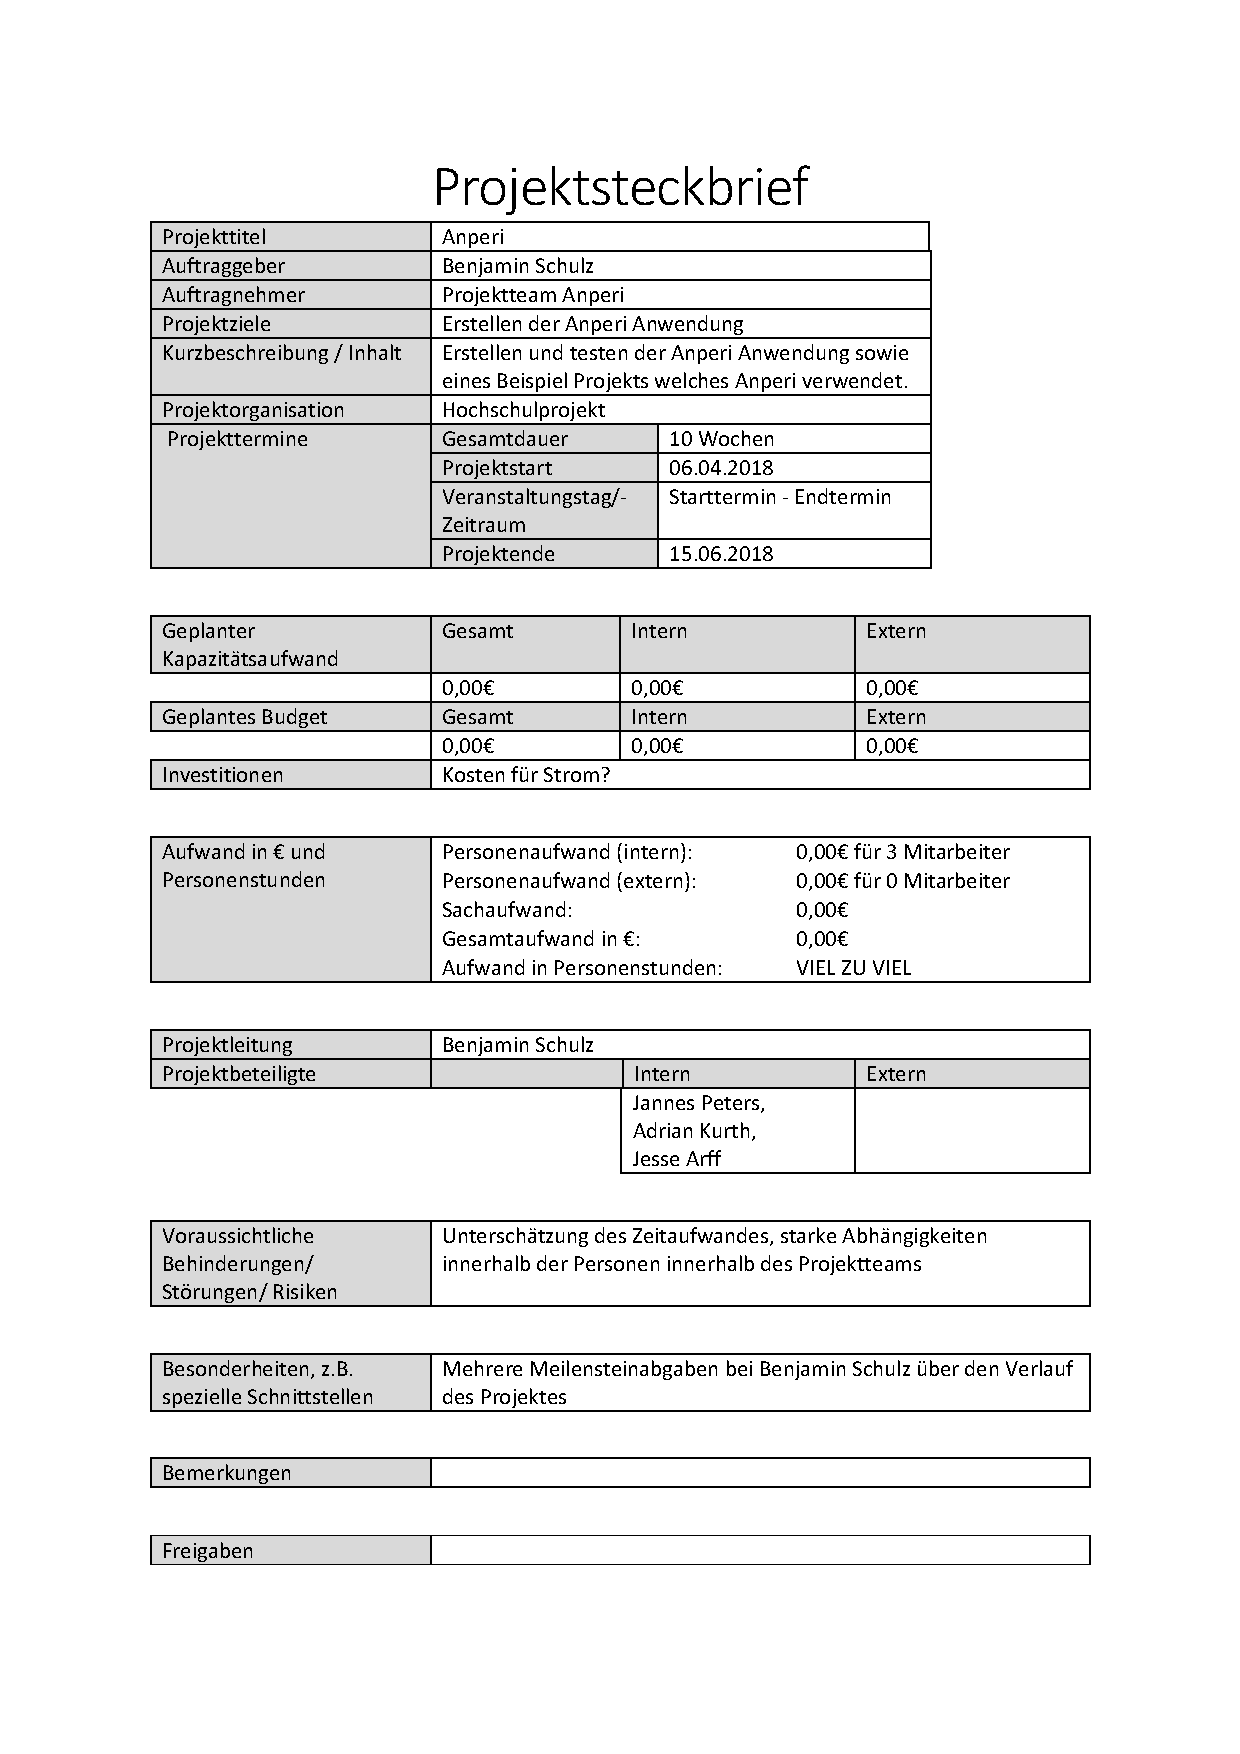
\includegraphics[scale=0.75]{Projektsteckbrief.pdf}
\includepdf[pages=2-, scale=0.75, pagecommand={\pagestyle{scrheadings}}]{Projektsteckbrief.pdf}

\section{Personenverteilung}
\subsection{Organigramm}
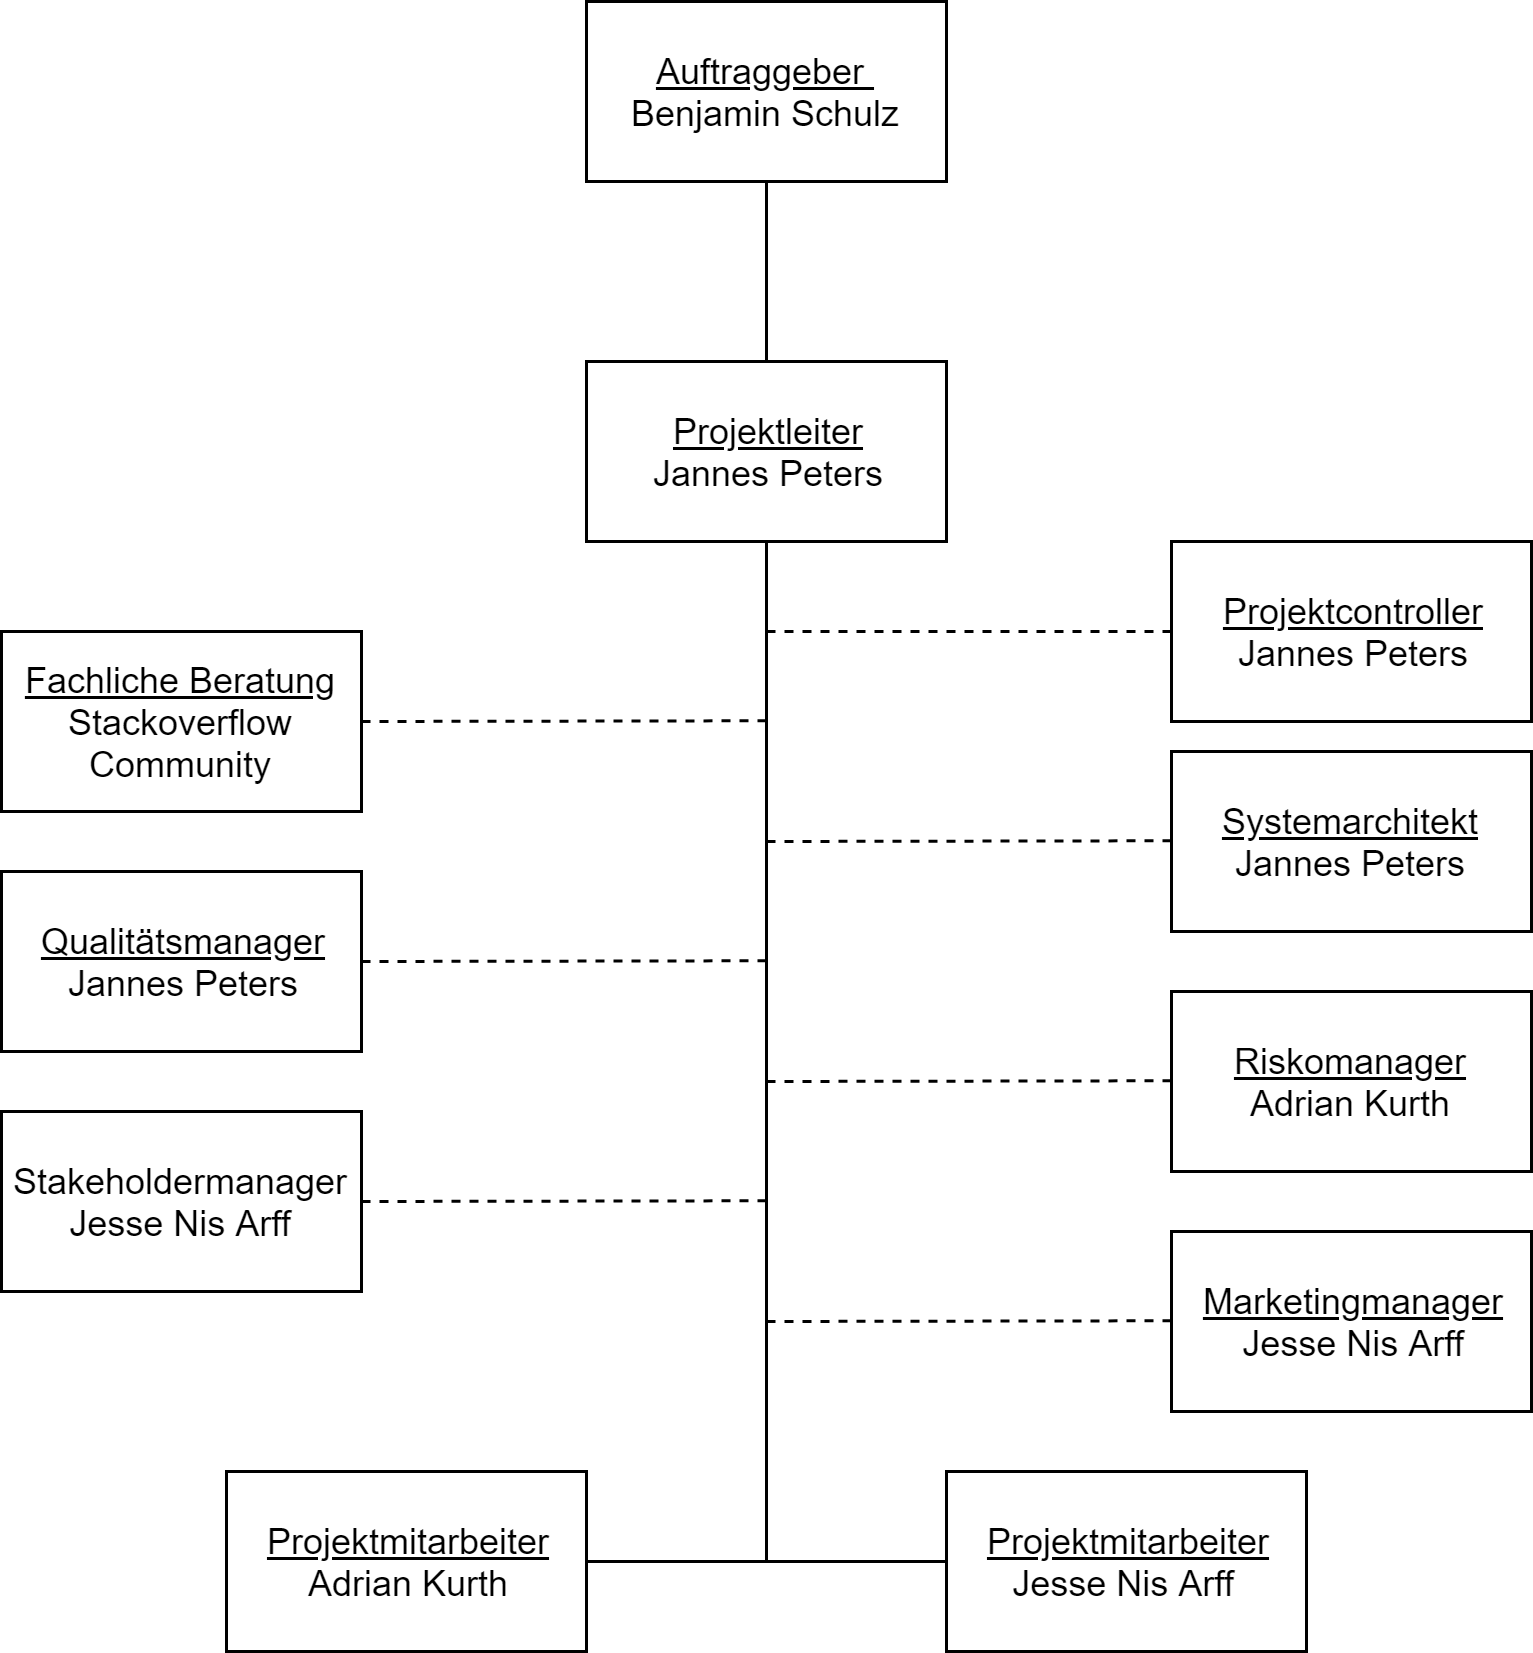
\includegraphics[scale=0.3]{Organigramm.png}
\subsection{Verantworlichtkeitsmatrix}
\begin{center}
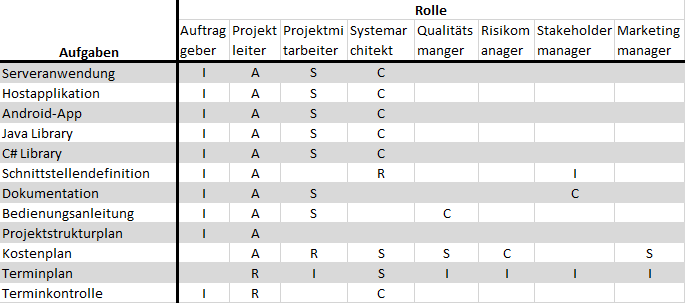
\includegraphics[scale=0.7]{RASCI.png}
\end{center}
\section{Phasenplan und Meilensteine}
\subsection{Phasenplan}
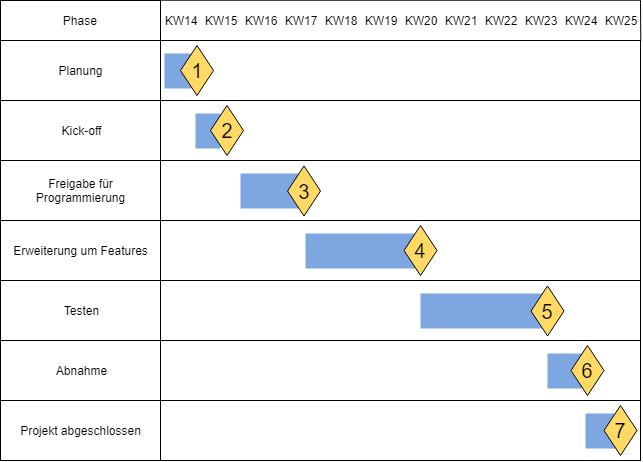
\includegraphics[scale=0.75]{Phasen.png}
\subsection{Meilensteine}
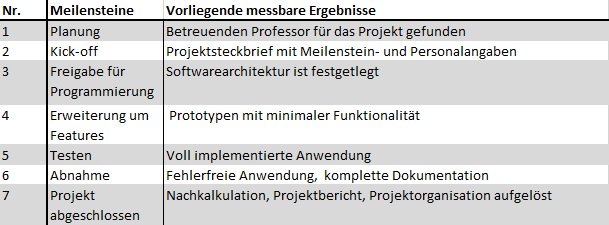
\includegraphics[scale=0.75]{Meilensteine.png}
\section{Projektstrukturplan}
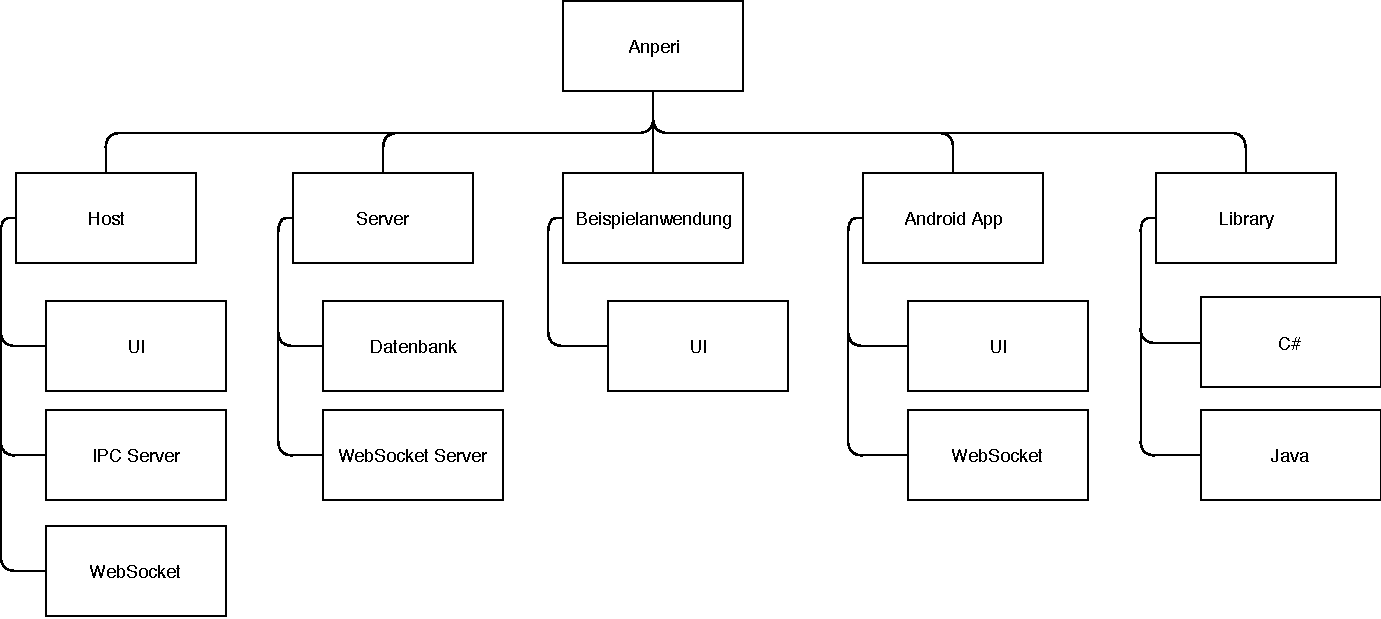
\includegraphics[scale=0.75]{PSP.pdf}
\subsection{Arbeitspaketbeschreibungen}






\end{document}